\documentclass[a4paper,parskip,BCOR=12mm,DIV=10]{scrbook}

%\usepackage{german}
\usepackage[utf8]{inputenc}
\usepackage{amsmath}
\usepackage{amsfonts}
\usepackage{amssymb}
\usepackage{mathtools}
\usepackage{faktor}
\usepackage{nicefrac}
\usepackage{listings}
\usepackage{enumerate}
\usepackage{dsfont}
\usepackage{remreset}
\usepackage{booktabs}
\usepackage{lettrine}
%\usepackage{txfonts}
\usepackage{varioref}
\usepackage{multirow}
\usepackage{rotating}
\usepackage{cancel}
\usepackage[pdfauthor={Joachim Breitner}]{hyperref}
\usepackage[capitalise]{cleveref}
% \usepackage{tikz}
% %\usepackage[tracking=true,kerning=true,spacing=true]{microtype}
% \usetikzlibrary{automata}
% \usetikzlibrary{decorations}
% \usetikzlibrary{snakes}
\usepackage{microtype}
\usepackage{framed}
\usepackage{caption}
\usepackage[normalem]{ulem}
\usepackage{tipa}

\usepackage{isabelle,isabellesym}

\usepackage[numbers,square]{natbib}
\bibliographystyle{amsplain}

% URLstyle
\urlstyle{rm}

% for \autoref
\newcommand{\examplename}{Example}
\newcommand{\lemmaname}{Lemma}
\newcommand{\remarkname}{Remark}
\newcommand{\corollaryname}{Corollary}
\newcommand{\definitionname}{Definition}
\newcommand{\algocflinename}{Algorithm}
\newcommand{\AlgoLineautorefname}{line}
\renewcommand{\chapterautorefname}{Chapter}
\renewcommand{\sectionautorefname}{Section}
\renewcommand{\subsectionautorefname}{Section}

% for \cref
\crefname{algocf}{Algorithm}{Algorithms}
\crefname{figure}{Figure}{Figure}

% vref settings
\vrefwarning
\def\reftextfaceafter {\unskip}%
\def\reftextfacebefore{\unskip}%
\def\reftextafter     {on the \reftextvario{following}{next} page}%
\def\reftextbefore    {on the \reftextvario{preceding}{previous} page}%
\def\reftextcurrent   {\unskip}%

% titlesec
\usepackage{titlesec}
\titleformat{\chapter}[display]
	{\sectfont\Large\filcenter}
	{\titlerule%[1pt]%
	 \vspace{1pt}%
	 \titlerule%
	 %\vspace{.4pc}%
	 \LARGE\MakeUppercase{\chaptertitlename} \thechapter}
	{1pc}
	{\titlerule
	 \vspace{1pc}%
	 \Huge}
% \titleformat{\chapter}[display]
% 	{\sectfont\Large}
% 	{%\titlerule%[1pt]%
% 	 %\vspace{1pt}%
% 	 %\titlerule%
% 	 %\vspace{.4pc}%
% 	 \LARGE{\chaptertitlename} \thechapter}
% 	{1pc}
% 	{%\titlerule
% 	 %\vspace{1pc}%
% 	 \sectfont%
% 	 \Huge}

%\pagestyle{headings}

% get rid of fourier fontenc warnings
% from http://newsgroups.derkeiler.com/Archive/Comp/comp.text.tex/2006-01/msg00679.html
\makeatletter
\let\my@@font@warning\@font@warning
\let\@font@warning\@font@info
\makeatother
%
\usepackage{mathpazo}
%\usepackage{fourier}
%\usepackage[math]{iwona}
%\usepackage{ccfonts}
%\usepackage{arev}
%\usepackage[garamond]{mathdesign}
%\usepackage{pxfonts}
%
\makeatletter
\let\@font@warning\my@@font@warning
\makeatother 

% Palatino: 5% mehr Zeilendurchschuss (laut KOMA-skript)
\linespread{1.05}

% Satzspiegel neu berechen
\recalctypearea

% Figures unabhängig vom Kapitel zählen
\makeatletter
\@removefromreset{figure}{chapter}
\renewcommand{\thefigure}{\arabic{figure}}
\@removefromreset{table}{chapter}
\renewcommand{\thetable}{\arabic{table}}
\makeatother

% Disable single lines at the start of a paragraph (Schusterjungen)
\clubpenalty = 10000
%
% Disable single lines at the end of a paragraph (Hurenkinder)
\widowpenalty = 10000 \displaywidowpenalty = 10000

% Remove skip between caption and figure.
\captionsetup[figure]{skip=0pt}

% listings
\lstset{language=Haskell
	,flexiblecolumns=True
	,columns=fullflexible
	,texcl=true
	,escapechar=!
	,basicstyle=\sffamily
	,stringstyle=\it
	,showstringspaces=false
	,literate={->}{$\to\,\,$}2 {→}{$\to\,\,$}2 {\\}{\textlambda}1
	}

% inputenc stuff
\DeclareUnicodeCharacter{03BB}{\textlambda}

% FrameSep default
\setlength{\FrameSep}{2pt}

\newcommand{\C}{\mathcal C}
\newcommand{\F}{\mathcal F}
\newcommand{\PR}{\mathcal {PR}}
\newcommand{\A}{\mathcal A}


\newcommand{\aC}{\widehat{\mathcal C}}
\newcommand{\aF}{\widehat{\mathcal F}}
\newcommand{\aPR}{\widehat{\mathcal {PR}}}
\newcommand{\aA}{\widehat{\mathcal A}}


\hyphenation{Karls-ruhe}

\author{Joachim Breitner}
\title{Control Flow in Functional Languages}
\subtitle{Formally taming lambdas}

\begin{document}
%\KOMAoptions{twoside=false}
\begin{titlepage}
\centering
\makeatletter
\textsc{\Large{Karlsruher Institut für Technologie}}\\
\vspace{.5em}
\textsc{\Large{Fakultät für Informatik}} \\
\vspace{4em}
{\Large \@author} \\
\vspace{2em}
{\large Student Research Project}\\
\vspace{2.5em}
{\sectfont\huge \@title }\\
\vspace{2em}
{\sectfont\Large \@subtitle }\\
% \vfill
% \begin{tikzpicture}[auto]
% \end{tikzpicture} \\
\vfill
Supervisors: \\
Prof. Dr. Gregor Snelting \\
Andreas Lochbihler \\
\vspace{2em}
{\large \@date }
\makeatother
\end{titlepage}
%\KOMAoptions{twoside=true}


\chapter*{Preface}

\lettrine I{n} his dissertation\cite{Shivers}, Olin Shivers introduces a concept of control flow graphs for functional languages, provides an algorithm to statically derive a safe approximation of the control flow graph and proves this algorithm correct. In this student research project, Shiver’s algorithms and proofs are formalized using the theorem prover system Isabelle.

This document starts with a concise overview of Shivers’ approach. Then the prototype in Haskell and the formalization in Isabelle is explained, stating where it differs from the original. Some of the more interesting choices, such as the use of \isatext{HOLCF}, in the formalization are explained. Special care was taken to make the appearance of the documents generated by Isabelle as similar to the original as possible. The tricks used to that end are explained. Some lemmas took several failed or unsatisfying attempts, which will not be hushed up. At last, some words about the used tools follow.


% \vfill
% \lettrine[nindent=1ex]I{} owe sincere thanks to Dr.\ Gabriela Schmithüsen, under whose guidance this thesis was created. She was always generous with time, advice, regular proof-reading, ideas and inspiration.
% 
% Moreover, I wish to thank Mareike Schmidtobreick and Pascal Maillard for proof-reading the final work.


\tableofcontents

\chapter{Taming Lambdas}

\lettrine F{unctional} languages, i.e.\ programming languages treat computations, including their context, as first class citizens, are harder to tackle by control flow analysis than imperative languages. For the latter, a function call names the function that will be called and a statical analysis can easily trace the control flow at that point. In functional languages, the callee can be a variable which, in turn, can contain any computation that was stored somewhere else in the program.

Additionally, such a stored computation is a \textit{closure}, i.e.\ contains the currently valid variable bindings. Therefore, a variable can have more than one current value at any given point in the program execution, where different closures see different values. This is an additional issue when trying to statically make statements about a function program’s control flow.

Shivers approaches this problem in his 1991 Ph.D.\ thesis, subtitled “taming lambdas”. He defines an exemplary functional language in \textit{continuation-passing style} (CPS). CPS means that the return value of functions can not return, but rather passed on to a continuation function, which has to be given as an argument. Consider for example the following code :
\begin{lstlisting}[language=Haskell]
main = print ((x + y) * (z - w))
\end{lstlisting}
In continuation-passing style, the operations \lstinline!+!, \lstinline!*!, \lstinline!-! and \lstinline!print! all take a continuation argument, and the \lstinline!main! function is being passed a top-level continuation: 
\enlargethispage{1em}
\begin{lstlisting}[language=Haskell]
main c = + x y (\xy. - z w (\zw. * xy zw (\prod. print prod c)))
\end{lstlisting}

\section{Syntax}

\begin{figure}
\begin{framed}
\begin{align*}
\text{PR} &\Coloneqq \text{LAM} \\
\text{LAM} &\Coloneqq (\lambda\ (v_1\ldots v_n)\ c) && [v_i\in \text{VAR},\, c\in\text{CALL}] \\
\text{CALL} &\Coloneqq (f\ a_1 \ldots a_n) && [f\in \text{FUN},\, a_i\in\text{ARG}] \\
&\phantom{\strut\Coloneqq\strut} (\text{\texttt{letrec}}\ ((f_1\ l_1)\ldots)\ c) && [f_i\in \text{VAR},\,l_i\in\text{LAM}\,c\in\text{CALL}] \\
\text{FUN} &\Coloneqq \text{LAM} + \text{REF} + \text{PRIM} \\
\text{ARG} &\Coloneqq \text{LAM} + \text{REF} + \text{CONST} \\
\text{REF} &\Coloneqq \text{VAR} \\
\text{VAR} &\Coloneqq \{\text{\texttt{x},\texttt{y},\texttt{foo},}\ldots\} \\
\text{CONST} &\Coloneqq \{\text{\texttt{3},\texttt{\#f},}\ldots\} \\
\text{PRIM} &\Coloneqq \{\text{\texttt{+},\texttt{if},\texttt{test-integer},}\ldots\} \\
\text{LAB} &\Coloneqq \{l_i,r_i,c_i,ic_p^j\ldots\}
\end{align*}
\end{framed}
\caption{CPS syntax}
\label{fig:syntax}
\end{figure}

The syntax definition is given in \vref{fig:syntax}. A Program (PR) is a lambda expression. Lambda expressions (LAM) abstract a call. Calls (CALL) either call a function with the given argument list or binds lambdas to names in a possibly mutually recursive fashion. Function values (FUN) can be lambda expressions, references to variables or primitive operations, while in argument positions (ARG), primitive operations are disallowed and constant expressions are allowed. References to variables (REF) name the referenced variable. There is a set of variable names (VAR). Constants (CONST) are either integers or \#f for a false value. A number of primitive operations (PRIM) are defined.

Although not given explicitly, every lambda, call, constant, variable reference and primitive operation is tagged with a unique label from the set LAB. These can be thought of as positions in the program source – for our purpose they are just an abstract set. Also we assume that programs are alphatised, i.e.\ each variable name $v$ is bound at exactly one position, whose label is given by $\text{\textit{binder}}\ v$. Additional \textit{internal labels} are added to this set for primitive operations, representing the internal call sites. For example the \texttt{if} primitive operation is being passed two continuation that might be called, one for the true case and one for the false case. Therefore, two internal labels are associated with this primitive operation.

\section{Standard Semantics}
\begin{figure}
\setlength{\FrameSep}{0pt}
\begin{framed}
\begin{align*}
\text{Bas} &= \mathds Z + \{\text{false}\} 
						& \PR &\colon \text{PR} \rightharpoonup \text{Ans} \\
\text{Clo} &= \text{LAM} \times \text{BEnv} 
						& \A &\colon \text{ARG}\cup\text{FUN} \to \text{BEnv} \to \text{VEnv} \to \text{D} \\
\text{Proc} &= \text{Clo} + \text{PRIM} + \{\text{\textit{stop}}\} 
						& \C &\colon \text{CALL}\to \text{BEnv} \to \text{VEnv} \to \text{CN} \rightharpoonup \text{Ans} \\
\text{D} &= \text{Bas} + \text{Proc}
						& \F &\colon \text{Proc}\to \text{D}^* \to \text{VEnv} \to \text{CN} \rightharpoonup \text{Ans} \\
\text{CN} &= \text{\textit{(contours)}} \\
\text{BEnv} &= \text{LAB} \rightharpoonup \text{CN} \\
\text{VEnv} &= (\text{VAR}\times\text{CN}) \rightharpoonup \text{D}\\
\text{Ans} &= (\text D + \{\text{\textit{error}}\})_\bot
\end{align*}
\end{framed}
\caption{CPS semantics domains}
\label{fig:semdoms}
\end{figure}


For this language, Shivers gives a denotational semantics for the above language, that is a partial function $\PR$ from the set of programs to the set of integers with an additional element indicating run-time errors. Following the structure of the syntax tree, he defines functions $\C$, $\F$ and $\A$ that evaluate call expressions, apply arguments to procedures and evaluate argument expressions, respectively. Their domains and ranges are given in \vref{fig:semdoms}.

the special value \textit{stop} is the continuation initially passed to the program. When this is eventually called, either in a CALL expression or as the continuation of a primitive operation, the evaluation comes to an halt and the argument to stop is the result of the evaluation. If a runtime error occurs (wrong number of arguments, callee not a procedure, undefined variable lookup), \textit{error} is returned.

The semantics functions are partial functions, indicated by the harpoon instead of the arrow and by the $\bot$ annotation of the set Ans. Functional programs are Turing-complete and therefore possibly non-terminating. For such programs, the semantics is defined to return $\bot$.

The evaluation context needs to be passed along the semantics functions and closures value need to encapsulate the context at the time the lambda expression is evaluated to a closure. The context information is separated into two pars here: The global \textit{variable environment} and the lexical \textit{contour environment} (or binding environment). The variable environment can store multiple values for each variable name. These are differentiated by a \textit{contour number} from the set CN. These can be thought of time stamps which are increased in every evaluation step. When a variable is bound to a new value, it is stored in the variable environment with the current contour number. The contour environment tells for each binding position (lambda or letrec expression) which contour counter is to be used when looking up a variable from that binding. By storing the contour environment within a closure and using it when evaluating the call inside the closure, the correct value for each variable binding is accessed.

The set CN of contours is not given explicitly here. Instead, we will treat it abstractly and only state the properties we expect from this set: There needs to be an initial contour $b_0$ and a function $nb \colon \text{CN} \to \text{CN}$ which generates a new contour. The set of contours is partially ordered and if $b$ is greater or equal than all allocated contours, then $nb\ b$ is strictly greater than all allocated contours. It is easy to see that the natural numbers with $b_0 = 0$ and $nb\ b = \text{Suc}\ b$ fulfill the requirements, but in the later proofs it will be convenient to choose other sets containing more information. 

\section{Exact nonstandard semantics}

At the moment we are not so much interested in the value a program returns but rather the calls that occur while evaluating the program. To that end the standard semantics introduced in the previous section are altered to calculate the \textit{call cache}. This is a partial map from call-site/contour-environment pairs to procedures. We therefore modify the domains of the semantics in \vref{fig:semdoms} as follows:
\begin{align*}
\text{CCache} &= (\text{LAB}\times\text{BEnv}) \rightharpoonup \text{Proc}\\
\text{Ans} &= \text{CCache}
\end{align*}

The semantics function definitions are extended to record the calls as they happen. For example, if $\C$ is applied to a call expression $(f\ a_1\ldots a_n)$ with label $c$ in context $\beta$ and $f$ evaluates to a procedure $f'\in \text{Proc}$, evaluation continues by applying $\F$ to $f'$ and the arguments. This returns a call cache, which is amended by the entry $(c,\beta) \mapsto f'$ to reflect the current call before the updated call cache is returned by $C$.

This semantics evaluates the program in full, just like the standard semantics, and is therefore unsuitable to be used in a static analysis. But it is the theoretic ideal that a statically calculated call cache will be compared against.

\section{Abstract nonstandard semantics}

Shivers then proceeds to define a nonstandard semantics that can be calculated statically. The trade off is that the call cache obtained now is just an approximation to the exact call cache, i.e.\ any possible call in the exact call cache will also be in the abstract call cache. The converse does not need to hold.

\begin{figure}
\setlength{\FrameSep}{0pt}
\begin{framed}
\begin{align*}
\widehat{\text{Clo}} &= \text{LAM} \times \widehat{\text{BEnv}}
						& \aPR &\colon \text{PR} \rightharpoonup \widehat{\text{Ans}} \\
\widehat{\text{Proc}} &= \widehat{\text{Clo}} + \text{PRIM} + \{\text{\textit{stop}}\} 
						& \aA &\colon \text{ARG}\cup\text{FUN} \to \widehat{\text{BEnv}} \to \widehat{\text{VEnv}} \to \widehat{\text{D}} \\
\widehat{\text{D}} &= \mathcal P(\widehat{\text{Proc}})
						& \aC &\colon \text{CALL}\to \widehat{\text{BEnv}} \to \widehat{\text{VEnv}} \to \widehat{\text{CN}} \rightharpoonup \widehat{\text{Ans}} \\
\widehat{\text{CN}} &= \text{\textit{(contours, finite)}} 
						& \aF &\colon \widehat{\text{Proc}}\to \widehat{\text{D}}^* \to \widehat{\text{VEnv}} \to \widehat{\text{CN}} \rightharpoonup \widehat{\text{Ans}} \\
\widehat{\text{BEnv}} &= \text{LAB} \rightharpoonup \widehat{\text{CN}} \\
\widehat{\text{VEnv}} &= (\text{VAR}\times \widehat{\text{CN}}) \rightharpoonup \widehat{\text{D}} \\
\widehat{\text{CCache}} &= (\text{LAB} \times \widehat{\text{BEnv}}) \to \widehat{\text{D}} \\
\widehat{\text{Ans}} &= \widehat{\text{CCache}}
\end{align*}
\end{framed}
\caption{CPS semantics domains}
\label{fig:abssemdoms}
\end{figure}

The abstract semantics $\aPR$ will run the program no longer in full detail. It will not keep track of actual values computed and conditional branches taken. Instead, it assumes that every branch of an \texttt{if} statement is possibly taken. Semantic values are now sets of possible procedures. \vref{fig:abssemdoms} gives the domains of the abstract semantics functions. 

After removing the plain values from our semantics domains, the remaining would all be finite – if  $\widehat{\text{CN}}$ were finite. This is the main trick to obtain a computable abstract semantics. If $\widehat{\text{CN}}$ is finite, there are only finitely many possible closures, procedures, binding environment, variable environments and call caches, and our function becomes computable.

Again, the choice of the set $\widehat{\text{CN}}$ is not fixed. Possible choices include a singleton set, resulting in “0th-order Control Flow Analysis” (0CFA) or the set of lambdas representing the call site a lambda was called from, resulting in 1st-order Control Flow Analysis (1CFA). The more information we store in the abstract contour counters, the more detailed our analysis will be, but also more expensive to calculate.

Because semantic values $\widehat{\text{D}}$ are now sets of procedures, when evaluating a call expression $(f\ a_1\ldots a_n)$, there is a set of possible procedure that $f$ can evaluate to, and $\aF$ will be called for each of them. The resulting call caches need to be joined using pointwise set union. Similarly, the continuations of primitive operations are sets of procedures, for all of which $\aF$ is called and the result is joined again.

\section{Main results}

The main results about these semantics functions are stated and shown in Shivers’ dissertation:
\begin{enumerate}
\item The call cache returned by the exact semantics is indeed a partial map,
\item the abstract semantics approximate the exact semantics and
\item the abstract semantics is computable.
\end{enumerate}

But before starting to proof these results, Shivers establishes that the recursive definitions he gave for $\F$ and $\C$ (and by analogy, $\aF$ and $\aC$) are sound. He proceeds in the standard way of turning a recursive definitions $f = F f$ for a function $f\in X$, where $X$ is a function space with a chain-complete partial order, into a functional $F\colon X \to X$. $F$ is then shown to be continuous and therefore has a least fixed point, which is used then defined to be $f$.
  

The need to show that the result of $\PR$ is a partial map is arises from the fact that, for an easier proof of continuity, Shivers changes the answer domain to be
\[
\text{Ans} = \mathcal P( (\text{LAB}\times\text{BEnv}) \times \text{Proc}).
\]
The actual proof is only outlined.

In contrast, the proof that $\aPR$ safely approximates $\PR$ is given in full detail. For any of the types Proc, D, $\text{D}^*$, BEnv, VEnv, CN and CCache, he defines an abstraction function (written $|\cdot|$) from the exact type to the corresponding abstract type. He also defines partial orders on the abstract types (written $\cdot \lessapprox \cdot$), expressing that one value is more specific than another value. The main result is then
\begin{quote}
\textbf{Theorem 6}: For any program $l$, call site label $c$ and binding environment $\beta$, we have
\[
|(\PR\ l)\ (c,\beta)| \lessapprox (\aPR\ l) (c,|\beta|).
\]
\end{quote}
The largest part of the proof is to show two similar statement relating $\F$ and $\aF$ (Lemma resp. $\C$ and $\aC$. Because these are mutually recursive, both statements are shown in one big step. The machinery to proof results about functions defined as fixed points is the fixed point induction: A predicate $P$ holds for the least fixed point of $F$ if the following three conditions are true:
\begin{itemize}
\item $P$ is an admissible predicate. This is closely related to continuity and states that if $P$ holds for each element of an infinite chain, it holds for the limit of the chain.
\item $P\ \bot$ holds.
\item If $P\ f$ is true, then $P\ (F\ f)$ is true.
\end{itemize}

The computability result is not shown explicitly for $\aPR$, but rather for general recursive equations of the shape
\[
f\ x = g\ x \cup f\ (r\ x)
\]
where each function invocation makes a local contribution to the result $g\ x$ and then recurses with a new argument $r\ x$. Shivers shows that in that case, the least fixed point is given by
\[
f\ x = \bigcup_{i=0}^\infty g\ (r^i\ x).
\]
If additionally the argument space is empty, the infinite union is actually only finite and the calculation is finished after a finite number of iterations.

The semantics functions $\aF$ and $\aC$ are nearly of this type, but they have a branch factor greater than one. Thus, for solution of an equations like
\[
f\ x = g\ x \cup \bigcup\{f\ x' \mid x' \in R\ x\}
\]
he introduces the \textit{powerset relative} of a function $h$ as $\uline h\ X\coloneqq \{h\ x \mid x\in X\}$ and transforms. the above equation to 
\[
\uline f\ X = \uline g\ x \cup \uline f\ (\uline R\ Y)
\]
to be able to apply the previous result.

The required steps to apply this result to the mutually recursive definitions $\aF$ and $\aC$ are not explained in the dissertation.

\chapter{The Haskell prototype}

\lettrine T{o} get a better understanding of the algorithms, a prototype was first implemented in Haskell. As the semantics are given in denotational style, they are easily translated into a functional program. The elements of the syntax definition of the CPS style language are directly turned into data type definitions.

At this point, we slightly deviate from the original: Shivers distinguishes the sets FUN and ARG as direct sums (cf.\ \vref{fig:syntax}) and later defines $\A$ on the union of FUN and ARG (cf.\ \vref{fig:semdoms}). This would be tedious and unwieldy to express in the Haskell type system, therefore we use one type VAL instead of FUN and ARG:
\begin{align*}
\text{VAL} &\Coloneqq \text{LAM} + \text{REF} + \text{PRIM} + \text{CONST}
\end{align*}
The change has very little effect on the following.

\section{Type system tricks}

As mentioned in the last chapter, most elements of the syntax carry a label. These labels need to be unique and every mention of a variable needs to carry the label of the variable’s binding position. To prevent the hypothetical user of the library from getting the labels wrong, the \textit{smart constructor} idiom was exploited.

A type alias is introduced to mark not-fully-constructed syntax tree values and prevent their use in other functions.
\begin{lstlisting}
newtype Inv a = Inv { unsafeFinish :: a } deriving (Show, Eq)
\end{lstlisting}
The accessor function \lstinline!unsafeFinish :: Inv a → a! is only to be used internally.

Now a value of type \lstinline-Inv Lambda- represents a lambda expression without correct labels. For each constructor there is a function (the smart constructor), taking the same arguments except the label, and building the unfinished value. For example, the smart constructor for lambda expressions is defined as
\begin{lstlisting}
lambda :: [Inv Var] -> Inv Call -> Inv Lambda
lambda vs (Inv c) = Inv $ Lambda noProg (map unsafeFinish vs) c
\end{lstlisting}
where \lstinline!noProg! throws, if it were evaluated, an exception:
\begin{lstlisting}
noProg :: a
noProg = error "Smart constructors used without calling prog"
\end{lstlisting}


There is only one function for public consumption that removes the \lstinline-Inv--wrapper, with signature \lstinline!prog :: Inv Lambda -> Prog!. It uses a state monad to hand out correct labels and keeps track of binding positions to correctly set the reference to the binding position. 

For additional convenience, the types \lstinline!Var!, \lstinline!Val! and \lstinline!Inv a! are made instances of the \lstinline!IsString! type class which allows the compiler together with the language extension \lstinline!OverloadedStrings! to turn string literals into values of these kinds, and similar with the \lstinline!Num!-instance for \lstinline!Val! to enter constants directly as literals.

\begin{figure}
\begin{framed}
\centering
\begin{lstlisting}
-- Returns the sum of the first 10 natural numbers            
ex3 :: Prog
ex3 = prog $ lambda ["cont"] $
        let_ [("rec", lambda ["p", "i", "c'"] $
                        app if_
                            [ "i"
                            , l $ lambda [] $
                                app plus ["p", "i",
                                    l $ lambda ["p'"] $
                                        app plus ["i", -1,
                                            l $ lambda ["i'"] $
                                                app "rec" [ "p'", "i'",  "c'" ]
                                            ]
                                    ]
                            , l $ lambda [] $
                                app "c'" ["p"]
                            ]
        )] $ app "rec" [0, 10, "cont"]
\end{lstlisting}
\end{framed}
\caption{Example Code}
\label{fig:sum10}
\end{figure}

A simple example program, returning the result of the worldshaking calculation $1 + 1$, is now written as
\begin{lstlisting}
ex2 :: Prog
ex2 = prog $ lambda ["cont"] $ 
        app plus [1, 1, "cont"]
\end{lstlisting}
instead of the much verbose
\begin{lstlisting}
ex2 :: Prog
ex2 = Lambda (Label 1) [Var (Label 1) "cont"] $
	App (Label 2) (P (Plus (Label 3))) [
		C (Label 4) 1,
	        C (Label 5) 1,
		R (Label 6) (Var (Label 1) "cont")].
\end{lstlisting}
A larger example is included in \vref{fig:sum10}, where the first ten natural numbers are added up.

\section{Pretty Printing and Graphical Output}

Another feature of the Haskell prototype is pretty-printing of an abstract syntax tree. It uses the standard pretty printing library of Haskell \cite{pretty} and renders the above example to the string “\texttt{(λ\ cont.\ (+)\ 1\ 1\ cont)}”. \vref{fig:prettyprint} shows the pretty printed presentation of the program in \vref{fig:sum10}.

\begin{figure}
\centering
\begin{framed}
\small
\begin{verbatim}

(λ cont.
   let rec = (λ p i c'.
                if i
                then (λ . (+) p i (λ p'. (+) i -1 (λ i'. rec p' i' c')))
                else (λ . c' p))
   in rec 0 10 cont)
\end{verbatim}
\end{framed}
\caption{Pretty-Printed Output}
\label{fig:prettyprint}
\end{figure}

After having pretty-printed the code, we wished a nicer presentation for the call caches returned by the semantics functions function. Recall that the call cache is a map from call sites, represented by labels, and binding environments to values. This can be turned into a map from labels to labels (hereby losing the context information) and thus arrows in the source code.

It turned out that the mapping from labels to coordinates in the source code is tricky to achieve: The used pretty printing library’s API has no way of marking positions in the result. An alternative would have been re-implementing the pretty printing library with this additional feature, but this would be out of scope for this project (even more than the graphical output). Instead we employed a hack abusing the wide range of characters that Unicode based strings provide: When pretty printing the code, labels (which are positive integers) are inserted as singe characters with a code point of U+100000 plus the number of the label. These are in the Private Use Area of the Unicode specification.

\begin{figure}
\centering
\begin{framed}
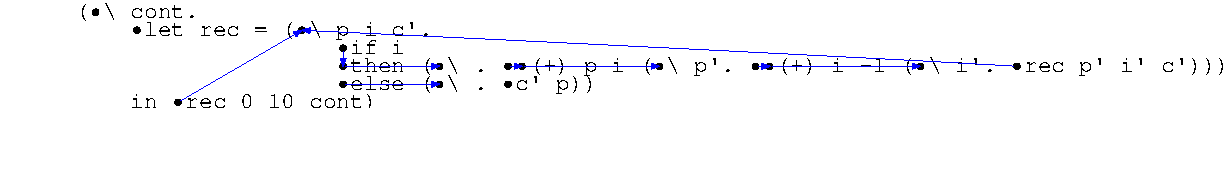
\includegraphics[width=\linewidth]{rendered-graph.pdf}
\end{framed}
\caption{The code annotated with the control cache}
\label{fig:ccgraph}
\end{figure}

After the pretty printer has laid out the code, we can gather the coordinates of all characters with code points larger or equal to U+100000 and replace them by a placeholder symbol (we chose $\bullet$). The pretty printed code is written to a PDF using the HPDF library\cite{HPDF}, which is implemented in pure Haskell. This gives us maximal control over the positioning and allows us to render the document without padding.

To draw the arrows, we want to use the graphviz suite\cite{Graphviz} which includes several graph layout mechanisms. From the edges given by the control cache and the label coordinates from the pretty-printed code a graph description in the dot-format is generated and rendered to PDF using the \texttt{neato} command. The two PDF files are now mapped onto each other using \texttt{pdftk}\cite{pdftk}. If everything went right, the arrows will begin and end exactly at the character that replaced the label. The result is included in \vref{fig:ccgraph}.

This was just a quick experiment and proof-of-concept. Obviously, this presentation has its weakness, as the reduced legibility of the code due to the arrows passing semi-transparently over the text.

Another conversion function is included that turn a program into the syntax used by Isabelle, to make it easier to obtain the example programs there as well.

\appendix

\bibliography{root}

\chapter*{Erklärung}

\lettrine H{iermit} erkläre ich, Joachim Breitner, dass ich die vorliegende Studienarbeit selb\-ständig
und ausschließlich unter Verwendung der angegebenen Quellen und Hilfsmittel verfasst
habe.
\vspace{20mm}
\begin{tabbing}
\rule{4cm}{.4pt}\hspace{1cm} \= \rule{7cm}{.4pt} \\
Ort, Datum \> Unterschrift
\end{tabbing}

\end{document}
